\chapter{Evaluation}

\label{Evaluation}

This chapter evaluates the System's capabilities and compares them to the requirements defined in Chapter 
\ref{Introduction}. It analyzes the System's performance and its ability to handle multiple audio streams 
simultaneously.

%----------------------------------------------------------------------------------------

\section{Streaming Capability \& Transcription Interval}

Since Whisper does not support real-time audio transcription, the System had to be designed to handle audio streams 
and utilize Whisper to transcribe slices of the audio stream. By implementing this feature, the System 
enhances the capabilities of Whisper and allows it to transcribe audio streams in near real-time.

The System slices the stream into chunks and transcribes them individually. The frequency of the transcription - 
and therefore the size of the chunks - is configurable using the "TranscriptionInterval" environment variable.

The following analysis compares the System's required transcription processing time with various amounts of 
simultaneously processed audio streams. The System runs on a machine with two Nvidia GeForce RTX 4070 graphics cards. 

The following table shows the average processing times for one, two, four, and eight simultaneous audio streams.

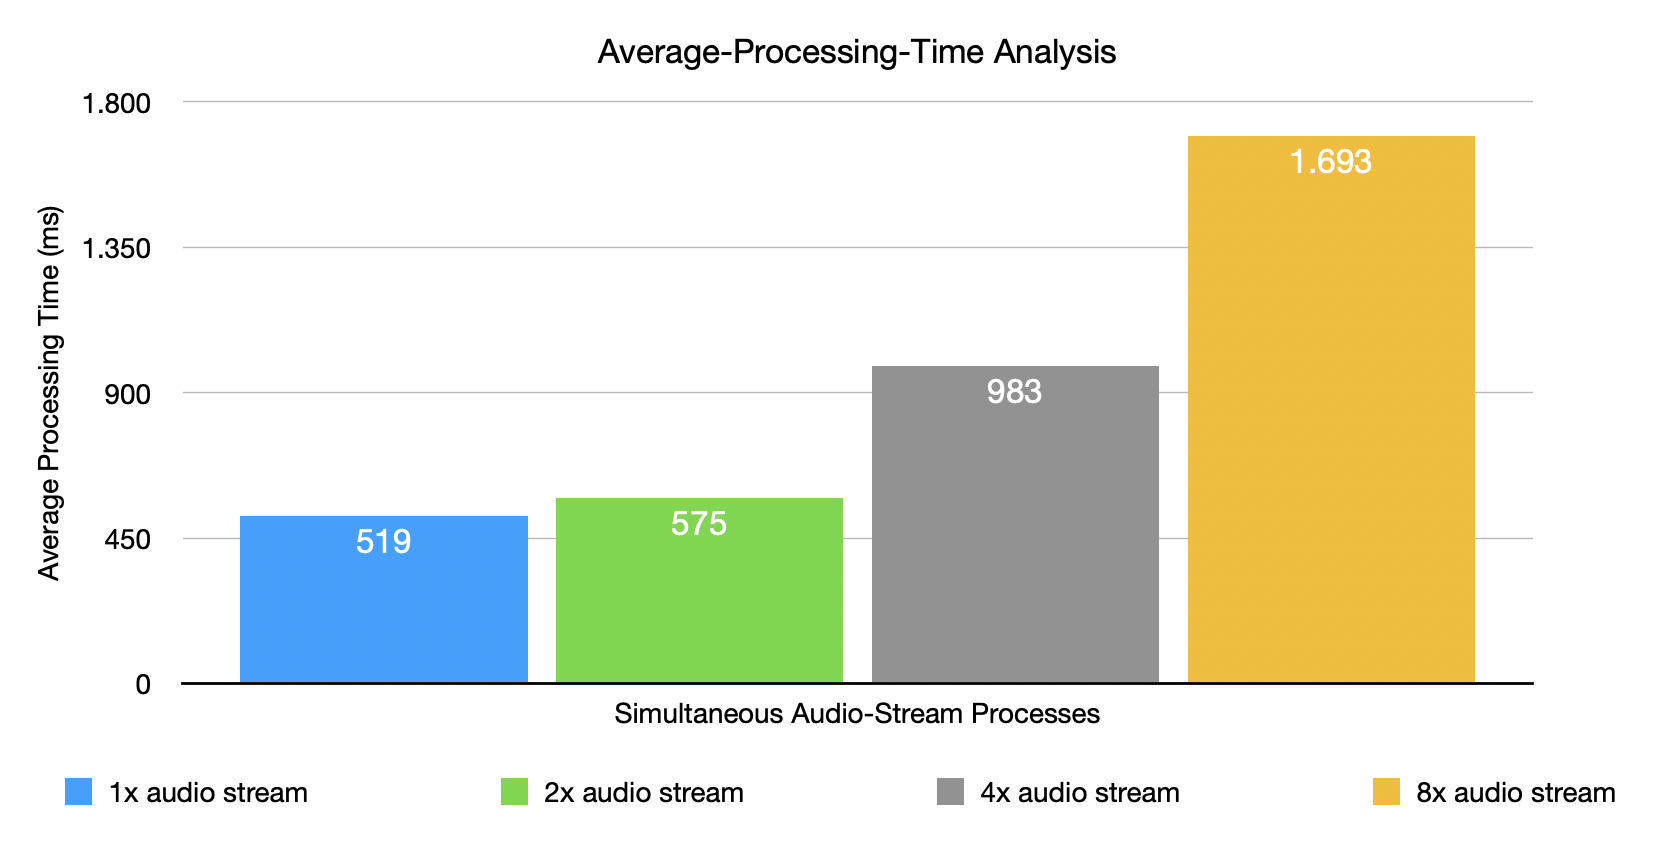
\includegraphics[scale=0.45]{Figures/avg-processing-times.png}

The diagram shows that the average processing time for one audio stream is 519 milliseconds. This would suggest that a 
transcription interval of about 520 milliseconds would be optimal for a hardware configuration like this. 

However, the diagram also reveals that the average processing time for two audio streams is 575 milliseconds. This 
seems unintuitive at first glance, but it is because the System utilizes a hardware setup with two graphics cards. 
The System can process two audio streams simultaneously, each on a separate graphics card. This results in a minor 
processing time increase for each audio stream since the System only shares CPU and data transmission resources between 
the two audio streams - not the GPU performing the transcription.

Looking at the average processing time for four simultaneous audio streams, we can see that it is 983 milliseconds. 
This significantly increases compared to the average processing time for two audio streams. This is because the System 
has to share the GPU resources between four audio streams - two on each graphics card. This results in a significant 
increase in processing time for each audio stream.

As shown in the last column of the diagram above, the average processing time for eight simultaneous audio streams is 
1,693 milliseconds. This significantly increases compared to the average processing time for four audio streams. 
This is because the System has to share the GPU resources between eight audio streams - four on each graphics card. 

\subsection{GPU Utilization}

The observation that the processing time increases are not doubled when the number of audio streams is doubled suggests 
that the utilization of the GPU is improved by running multiple audio transcriptions simultaneously. The GPU is only 
partially utilized when processing a single audio stream. A second, third, or fourth audio stream can utilize more GPU 
resources even though the processing time increases overall.

\subsection{1500ms Transcription Interval}

To ensure the System can handle multiple audio streams simultaneously, it uses a transcription interval of 1500 
milliseconds by default. This transcription interval is configurable using the "TranscriptionInterval" environment 
variable. The transcription interval is the time between two transcriptions of the same audio stream.

1500 milliseconds is a good default value for the transcription interval because it allows the System to support up to 
eight simultaneous audio streams on a machine with two Nvidia GeForce RTX 4070 graphics cards. When all eight audio 
streams are active, the System has a processing time more significant than the transcription interval. To prevent this, 
the System awaits the results of the previous transcription before starting a new one for the same audio stream. This 
ensures that the System can handle up to eight simultaneous audio streams without requesting more resources than are 
available.
